\chapter{Implementação paralela dos algoritmos}

Como descrito anteriormente, o processamento de cada quadrícula de dados é feita de forma independente uma da outra, fazendo com que a implementação paralela desses algoritmos seja algo natural a se fazer. Entretanto, existem alguns problemas a serem enfrentados para o sucesso dessa tarefa, especialmente ao usar a plataforma CUDA.

Nesse capítulo serão analisadas as principais etapas e dificuldades das implementações paralela em OpenMP \cite{openmp_guide} e CUDA \cite{cuda_guide} dos algoritmos Filtro de Lanczos e Teste de Monte Carlo, apresentados no capítulo \ref{cap:algs_atmosfericos}.

\section{Implementação em OpenMP}

A maior vantagem em se usar as bibliotecas OpenMP \cite{openmp_guide} para implementar soluções paralelas desses algoritmos é a facilidade. Isso se dá primeiramente pelo fato de que não é necessário um tratamento especial da memória, diferente da implementação em CUDA, e principalmente por se tratar da adição de pouquíssimas linhas de código com a função de apenas especificar como a função em questão deve ser paralelizada.

Esses fatores são especialmente importantes no caso dos algoritmos estudados pois o fato de não haver mudanças mais profundas no código há uma maior confiança nos resultados obtidos. Além disso, o código é capaz de rodar em qualquer processador e não é necessário a  reconfiguração de nenhum parâmetro para que a execução em máquinas diferentes seja a melhor possível, pois a configuração do número de threads já é feita durante a execução. Isso faz com que seja muito fácil o uso dessa solução por parte dos pesquisadores em qualquer máquina.

Porém, como será descrito mais a frente, essa solução possui uma escalabilidade muito pequena, e em alguns casos o tempo de execução pode ser até maior do que a implementação sequencial. Por estas razões essa implementação será usada apenas como referência.

\section{Implementação em CUDA}

Diferente da solução com base em OpenMP, a implementação em CUDA \cite{cuda_guide} possui uma grande escalabilidade e reduziu significantemente o tempo de execução em todos os testes realizados. Porém, a sua implementação necessita de muito mais cuidados, além de uma placa-de-vídeo que suporte a tecnologia CUDA.

CUDA é uma arquitetura criada pela empresa NVidia que utiliza placas-de-vídeo para executar algoritmos em paralelo, utilizando as centenas de núcleos de processamento presentes nessas placas, também chamadas de GPUs. Dentro do contexto CUDA essa placa é chamada de device e a máquina em que esse device está acoplado é chamada de host.

Outros fatores importantes a se notar é que essas placas possuem uma memória própria e que a cópia da memória entre o host e o device não é feita automaticamente a quantidade, além de que a quantidade dessa memória existente é limitada e não há a possibilidade de expansão. São esses fatores que fazem com que a implementação seja mais difícil, especialmente no caso dos algoritmos estudados os quais, como já explicado, necessitam de uma grande quantidade de memória.

\subsection{Proposta de solução}\label{cap:proposta_solucao}

Uma solução para possibilitar o uso desses algoritmos em qualquer plataforma CUDA, independente do tanto de memória disponível, é processar esses dados em ciclos de processamento, ou seja, processar apenas uma parte dos dados de entrada a cada ciclo. Porém os mesmos são originalmente organizados de forma que os valores dos eixos X e Y fiquem juntos, fazendo com que os valores de uma quadrícula no eixo do tempo fiquem separados, o oposto do que seria o ideal. Isso não é nenhum obstáculo quando pensamos numa execução sequencial do algoritmo, onde a quantidade e facilidade de acesso à memória é maior, mas impossibilita a ideia de ciclos de processamentos, pois impede que os mesmos sejam repartidos.

%%%%%%%%%%%%%%%%%%%%%%%%%%%%%%%%%%%%%%%%%%%%%%%%%%%%%%%%%%
% FIGURA
\begin{figure}[H]
\centering
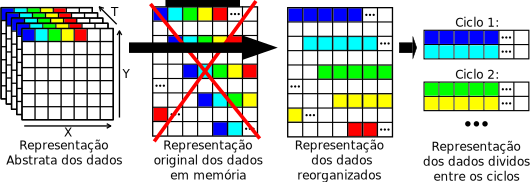
\includegraphics[width=0.8\textwidth]{Imagens/organizacao_dados/organizacao_dados.png}
\caption{Organização dos dados}
\label{fig:organizacao_dados_2}
\end{figure}
%%%%%%%%%%%%%%%%%%%%%%%%%%%%%%%%%%%%%%%%%%%%%%%%%%%%%%%%%%

Para contornar isso foi utilizado uma função de leitura que armazena os dados na memória do Host de forma que a série de tempo de cada quadrícula seja contínua, como demonstrado na figura (\ref{fig:organizacao_dados_2}), assim sendo possível copiar pedaços separados desse dado para o device. Além disso, ao invés da estrutura de matriz, foi usado a estrutura de um vetor comum para armazenar esses valores e funções auxiliares para calcular a posição na memória em que se inicia os dados de cada quadrícula. Essa decisão ainda facilita a cópia de dados entre a memória do Host e do Device.

\subsection{Implementação da solução}\label{cap:implementacao_solucao}

Em teoria essa tarefa seria a mais difícil do processo de implementação do algoritmo em CUDA, porém foi a que menos precisou de ajustes. Na função que implementa o algoritmo em si as únicas alterações necessárias foram remover o loop de incremento das quadrículas a serem processadas, necessário na versão sequencial, e adicionar o cálculo que defini qual quadrícula cada um dos núcleos de processamento do device será responsável por processar. Essas alterações estão detalhadas na figura \ref{fig:comparacao_codigo_padrao}, juntamente com as necessárias para implementar a solução em OpenMP.

%%%%%%%%%%%%%%%%%%%%%%%%%%%%%%%%%%%%%%%%%%%%%%%%%%%%%%%%%%
% FIGURA
\begin{figure}[H]
\centering
\includegraphics[width=0.7\textwidth]{Imagens/comparacao_codigo/comparacao_codigo_padrao.png}
\caption{Comparação da função que implementa o algoritmo}
\label{fig:comparacao_codigo_padrao}
\end{figure}
%%%%%%%%%%%%%%%%%%%%%%%%%%%%%%%%%%%%%%%%%%%%%%%%%%%%%%%%%%

Foi a função \texttt{Main} do código em C que sofreu as maiores mudanças, como pode ser visto na figura \ref{fig:comparacao_codigo_main}. Porém, grande parte dessas alterações foram apenas para adicionar as premissas básicas de todo programa, como alocação e inicialização de memória, no contexto do CUDA. As outras modificações foram a adição das funções de cópia de memória entre Host e Device e um loop para controlar os ciclos.

Esses ciclos foram pensados para o caso da memória total necessária para armazenar os dados de entrada e saída for maior do que o total de memória disponível no device. Para que esse método funcione, além da organização dos dados previamente descrita, foi criado um pequeno algoritmo para dividir igualmente o processamento entre os vários ciclos. Dentro de cada um desses ciclos as seguinte ações são executadas, em ordem:

\begin{enumerate}
\item Cálculo da posição de início da cópia dos dados de entrada;
\item Cópia dos dados de entrada do Host para o Device;
\item Execução do algoritmo em questão;
\item Cálculo da posição de início da cópia dos dados de saída;
\item Cópia dos dados de saída do Device para o Host;
\end{enumerate}

Todas essas ações possuem relações diretas com as ações consideradas praticamente obrigatórias em todas os programas escritos em C. São elas: leitura dos dados de entrada, execução do algoritmo de processamento, escrita dos dados de saída. Portanto, com exceção das alterações obrigatórias para adaptar o programa à plataforma CUDA, não foi feito nenhuma modificação ou otimização no código que implementa os algoritmos em si.

%%%%%%%%%%%%%%%%%%%%%%%%%%%%%%%%%%%%%%%%%%%%%%%%%%%%%%%%%%
% FIGURA
\begin{figure}[H]
\centering
\includegraphics[width=0.7\textwidth]{Imagens/comparacao_codigo/comparacao_codigo_main.png}
\caption{Comparação da função \texttt{Main}}
\label{fig:comparacao_codigo_main}
\end{figure}
%%%%%%%%%%%%%%%%%%%%%%%%%%%%%%%%%%%%%%%%%%%%%%%%%%%%%%%%%%